\scanpage{34}\mspage{33}
% @opening
sub-country ; Ditto This term is improper. Unless reserving the name of ``country'' for \deleted{\uline{all}} \inserted{more or less} systems $(M,\ll,\unsure{\mathcal R|\mathcal Q}_{M})$. I will still restate a few axioms, \unsure{potentially|particularly} crucial
% @cont1

\margin{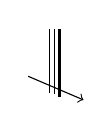
\begin{tikzpicture}[x=.6cm,y=.6cm]
\draw (0,1.5)--(0,.15); \draw (.10,1.5)--(.10,.12); \draw[line width=1pt] (.22,1.5)--(.22,.06);
\draw[->] (-.45,.50)--(.72,0);
\end{tikzpicture}}
\uline{Cont} \uuline{1} The relation ``$X\leq Y$'' ($\Longleftrightarrow X\ll Y$ and $X$ compatible $Y$) is an order relation
% @m1
% slanted
\margin{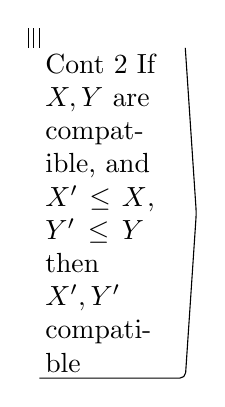
\begin{tikzpicture}
\node[inner sep=2pt,text width=1.7cm,align=left] (m34) {\uline{Cont} 2 If $X,Y$ are compatible, and $X'\leq X$, $Y'\leq Y$ then $X',Y'$ compatible};
\draw (m34.north west)--++(0,.25); \draw ([xshift=-.07cm]m34.north west)--++(0,.25); \draw ([xshift=-.14cm]m34.north west)--++(0,.25);
\draw[rounded corners=2pt] (m34.north east)--([xshift=.14cm]m34.east)--(m34.south east)--(m34.south west);
\end{tikzpicture}}
% @fig2

\deleted{Cont 2} \inserted{\textcircled{\scriptsize Fig 2}} \deleted{Every} If $F\in\mathcal F$, two elements \inserted{$X,Y$} of $F$ are compatible, and $F$ is a \uline{closed} subset of the set $M(\unsure{\leq|\ll})$.
% @fig3

\deleted{\unsure{Cont 3|Cont 4}} \inserted{\textcircled{\scriptsize Fig 3}} If $F$ \deleted{and $G$ are two} \inserted{is a} figure, every subset $F'$ of $F$ which is closed, is a figure (called a \uuline{subfigure}).
% @m2
% slanted
\margin{\uline{NB} If \deleted{\unsure{$F,G$}} $F',F$ are figures such that $F'\subset F$, then $F'$ is closed in $F$, because of Fig 1}
% @empty
% The text enclosed by the long contour is also the conclusion of the lower Cor.
\figure{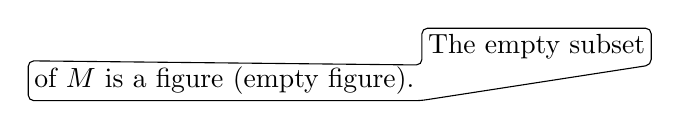
\begin{tikzpicture}[remember picture]
\node[anchor=south west,inner sep=2pt] (emptystart) at (5.0,.20) {The empty subset};
\node[anchor=west,inner sep=2pt] (emptyrest) at (0,0) {of $M$ is a figure (\uuline{empty figure}).};
\draw[rounded corners=2pt] (emptyrest.west) -- (emptyrest.north west) -- (emptystart.south west) -- (emptystart.north west) -- (emptystart.north east) -- (emptystart.south east) -- (emptyrest.south east) -- (emptyrest.south west) -- cycle;
\end{tikzpicture}}
% @fig1

\deleted{\unsure{Cont 3|Cont 4}} \inserted{\textcircled{\scriptsize Fig 1}} If $X\in M$, the set \inserted{$F_{X}=M_{\leq X}$} of $Y\in X$ \deleted{such} \deleted{\unsure{that}} that \unsure{$Y\leq X$} is a figure, which is called the ``\uuline{elementary figure}'' \unsure{defined} by \uline{the} multiplicity $X$.
% @cor

\uline{Corollary}. \inserted{(of Cont 2 and Cont 4)} If $M\neq\varnothing$, \tikz[remember picture,baseline]{\coordinate (corend) at (0,.15); \draw[overlay,->] (emptyrest.west) .. controls +(-1.2,-1.6) and +(-.4,-.8) .. (corend);}
% @nb

\uline{NB} If $M=\varnothing$, \deleted{If $M=\varnothing$} the axiom \uline{Fig \unsure{3|4}} becomes vacuous -- we replace it by \unsure{:} \deleted{the subset} \deleted{the \unsure{empty subset of|empty subset is} $M$} the only subset of $M$ (namely the empty subset) is a figure.
% @cancelled

\deleted{\uline{Corollary} (of \uline{Fig 1} and \deleted{\unsure{the}} \uline{Fig 2}) If \deleted{$X$}, $Y,Z$ are such that \unsure{$Y,Z$}$\ll X$, and if $Y,Z$ are compatible with $X$, then are among \unsure{themselves}}
